% !TEX root = ../../fyp.tex
\documentclass[../../fyp.tex]{subfiles}

\begin{document}

Consider a sub-space composed of all Out-Of-Vocabulary(OOV) tokens in the training and testing datasets. We assume the existence of an arbitrary amount of knowledge distributed across this sub-space which may or may not have a direct influence on the sentiment of the context of an OOV token where it appears. Ideally, a model learns an accurate representation of the weight of this influence during training, with each time it encounters the token. OOV tokens hinder this process in two ways; first, OOV words are, by definition, scarce within a given vocabulary and therefore provide limited opportunities to construct and optimize an accurate representation. Second, when these tokens are encountered, the effect on the sentiment of their context is attenuated when compared to other, more frequent, tokens for which the model has numerous opportunities to fine-tune its understanding of token's consequential effect on the task at hand. In our OOV sub-space, this is analogous to the information contained therein being spread too thin across all the tokens comprising it. 

The motivation underlying the following work is to investigate whether this OOV sub-space can be effectively encoded into a smaller number of clusters, each composed of tokens with shared properties, ideally relating to the sentiment information each carries. Since the information contained within the OOV sub-space is finite, the degree to which such an approach would be effective is modulated by the cluster-cardinality, which determines the range of information we intend to encapsulate in each cluster.

We use our framework to construct a series of experiments consisting of a baseline, followed by variations on the aforementioned range of information. This is achieved through the OOV policy parameter, specifically the OOV-train-threshold and OOV-bucket parameters. Combined, these parameters provide a mechanism by which to cluster single OOV tokens, encountered both at the training and testing stage, into unique vector representations which are subsequently updated in the model's training process. 

This section provides a detailed description of the experiment setup and motivations behind the specific choices made, followed by an analysis of the corresponding results.

\subsection{Experiment Setup}

When preparing these experiments, our principal consideration is the resource overhead involved in each configuration as a function of both time and cost. Addressing the latter, we select a model from our previous reproduction studies with the least complexity, namely the TD-LSTM approach \cite{tang2016b}. This model consumes the least amount of resources in training while maintaining a sufficient degree of aptitude for TSA, particularly in the social-media network domain in conjunction with the common-crawl 840b GloVe embeddings. 

Additionally, to obtain more in-depth insight into the effects of these OOV strategies, we seek to maximize the vocabulary size of a dataset, thereby increasing the absolute number of OOV tokens present. Towards this end, we use the nakov dataset (\S\ref{ds:nakov}), which has a considerably higher vocabulary compared to the Dong (\S\ref{ds:dong}) dataset while retaining the same social-media domain.

The above limitation of time is the tokenization and mapping processes being contingent on the OOV parameters we are investigating. As described in \S\ref{sec:data_module}, these tasks fall under the responsibility of the data module. They must be carried out locally before being delegated to the cloud. Furthermore, the time required for these tasks, in particular, mapping each token to its respective index in the embedding matrix, increases drastically with the size of both embeddings and the vocabulary of the dataset.

Were we to tackle this problem using a different embedding, we expect a notable decrease in the model's performance as observed in the reproduction experiment. The fact that this embedding variant is the only one that is case-sensitive is also intentional, as this adds a degree of precision when matching tokens, which increases the probability of a token being OOV. 

Therefore, we must address the alternative bottleneck, the dataset, by limiting its vocabulary size. This is in direct opposition to our motivation in choosing this dataset, however, and an overly-aggressive approach here negates any insights we may have otherwise obtained by using this dataset as opposed to Dong.

To account for these circumstances, we employ the framework's re-sampling function to downsample the original training dataset into a smaller, evenly distributed version. Notably, we exclude the testing dataset from this process, reducing the amount of OOV tokens that the model may have otherwise encountered in training while maintaining the same amount of OOV tokens in testing. Moreover, this approach ensures that the model is exposed to an equal number of positive, neutral, and negative samples in training.
The resultant dataset reduces the time required by an average of 75\% (2hrs vs. 30mins)

We identified several irregularities in the Nakov dataset upon further inspection. Notably, this dataset lacks any specific offset value, which precisely indicates the location of a target in a sentence. We design the framework to address this issue by automatically determining the offset using a standard string search when these are not provided. Despite this, multiple occurrences of the target string in a sentence obscure this process, since there is no means of discerning the intended target.

One approach to this problem is to include the sample multiple times for each target occurrence. However, this imposes the need for a memory element when parsing data to recall if any previous target mentions in a sentence have been accounted for. We determine the added complexity in this approach to be excessive for the portion of the samples affected. 

We instead implement a stricter matching function using regular expressions at a minimal additional overhead cost to the parsing. This prioritizes instances of the target surrounded in word boundaries and falls back to the more straightforward string matching approach when this returns no results. We discard the samples for which this approach is still unable to determine the target location in the sentence with certainty. 

A minority of multi-word targets in the dataset are separated by characters in the sentence inconsistent with the target entity. The confounding variables surrounding the small subset of samples exhibiting this issue did not merit a generalized approach. Therefore these samples were also discarded from the dataset. Finally, we map the original 5-degree sentiment classes of the dataset to 3-degrees as outlined in \S\ref{sec:datasets}.

\subsection{Model Parameters}
For each OOV policy, we assess the performance of the model with slight variations to the default parameter set used in the reproduction studies, since this is a novel dataset, to identify the ideal parameter set for it. These variations include a learning rate of 0.1 as opposed to 0.01 and increasing the hidden unit count of the LSTM to 300 as opposed to 200, as well as a third configuration comprising both. We report results on the best performing parameter set across all OOV policy configurations. 

\subsubsection{OOV Train Threshold}
The first parameter is the OOV training threshold level, which stipulates a minimum number of times an OOV token must be encountered during training to be assigned its vector in the embedding matrix. We refer to the number of tokens that meet this threshold as a fraction of the total number of OOV token in the training dataset as the train-time OOV coverage. Consequently, a threshold value of 1 results in 100\% train-time OOV coverage. 

Any value greater than 1 drastically reduces this coverage as in most datasets, the vast majority of OOV tokens appear only once. The framework reserves the 0 value to denote the condition where all OOV tokens in training are ignored and subsequently bucketed, effectively setting train-time OOV coverage to 0\%.

With every increment beyond a threshold of 1, however, we observe a rapid decrease in the train-time OOV coverage. For these reasons, we limit our experiments to a threshold value of 2 (6.12\% cov.) and 3(2.28\% cov.). Values beyond this are nearly indistinguishable from the 0-valued case (0\% cov.). 

\subsubsection{OOV Test Bucket Number}
The second OOV policy parameter determines the number of buckets in which test-time OOV tokens are distributed. These buckets are each assigned a vector in the embedding space. They are analogous to the clusters, as mentioned earlier in our OOV sub-space. Consequentially, this parameter is inversely proportional to the amount of information each bucket is expected to encapsulate on average. Therefore, a common approach of assigning all OOV words to a unique randomly initialized vector is represented by a value of 1, which is also the default value used in our reproduction studies. 

When assigning each token to a bucket, we employ the native hashing function, which is included in the Tensorflow library. 
We adopt a principled approach to this idea, investigating a broader range of values spanning 3 different orders of magnitude. Doing so identifies the potential degree to which this strategy can manifest positive downstream effects on performance. 

We leave further research into more granular fine-tuning of this value as well as more sophisticated hashing algorithms that assign tokens to buckets for future work. 

\subsection{Results and Observations}

We adopt a similar approach to our reproduction studies, to a lesser extent to account for the increase in the number of experiments. Each experiment configuration is run 4 times and we gauge the performance of each using the macro-F1 score to account for the class imbalance in the testing dataset. We find the best performing parameter set for this modified Nakov dataset is the variant with 300 hidden units and a learning rate of 0.1. We speculate that with the increased vocabulary in the Nakov dataset, the model can effectively leverage the additional parameters to produce a more accurate representation of the dataset. Moreover, the faster learning rate may be a means by which the model is able to extract more information from the reduced sample size of the training dataset by amplifying the effect of each. 

\begin{figure}[!ht]
	\centering
	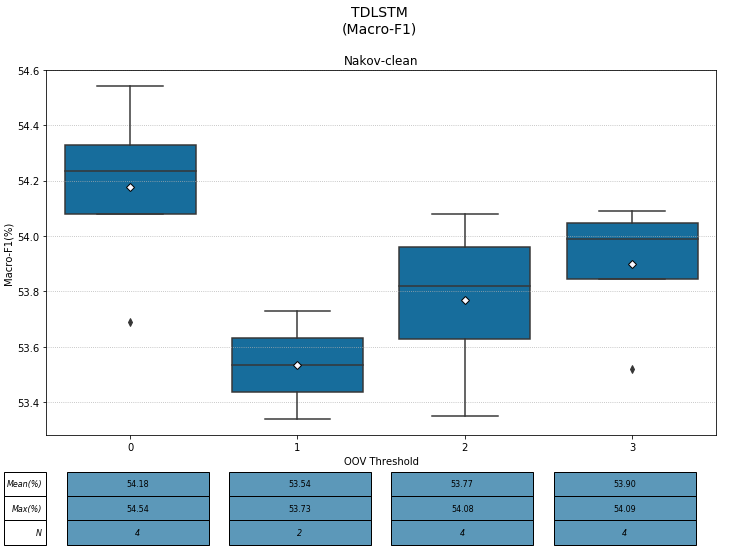
\includegraphics[width=\textwidth]{oov_threshold_ablation.png}
	\caption{Results obtained with varying OOV training threshold parameters. (OOV Buckets = 1)}
	\label{fig:oov_threshold_ablation}
\end{figure}

We illustrate the results of different threshold level, while maintaining the bucket parameter at 1, in \ref{fig:oov_threshold_ablation}. We observe the most pronounced improvement when $T=0$, which disregards all OOV tokens in training. We believe the larger deviation of this configuration results from the minuscule effect on train-time OOV coverage that the other values have compared to $T=1$. More surprising however is the polarity of this difference, which suggests that it is more beneficial to disregard OOV tokens at training altogether. 

This may indicate that due to the low occurrence rate of OOV tokens, and the natural distribution of words in languages, there lacks sufficient contextual information to embed the significant of the OOV token in isolation. This effectively reduces the added vectors to noise, which would be reduced by increasing threshold values above 1, which can be observed in the slight gradual improvement of macro-f1 scores in \ref{fig:oov_threshold_ablation}  Recall that in this configuration, we set the OOV buckets to 1, therefore when $T=0$ all training OOV tokens are subsequently grouped under a single OOV bucket. Increasing the granularity of this strategy with additional buckets may further improve the performance of this approach.

\begin{figure}[!ht]
	\centering
	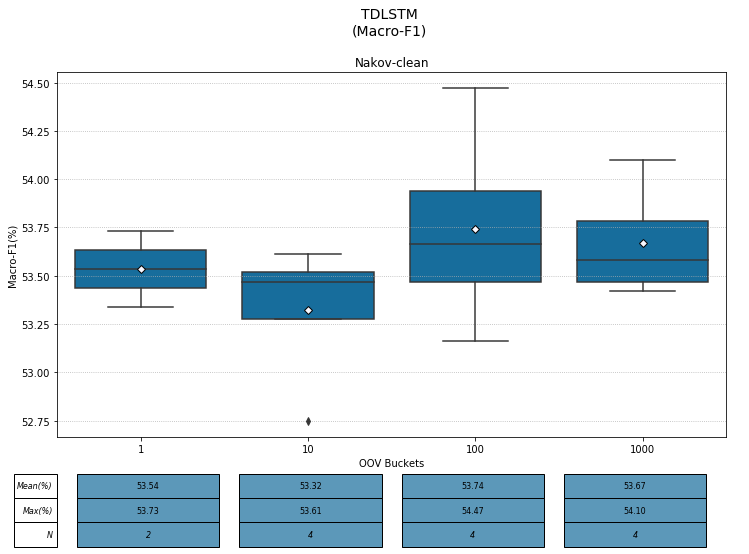
\includegraphics[width=\textwidth]{oov_buckets_ablation.png}
	\caption{Results obtained with different numbers of test time OOV buckets. (OOV Train Threshold = 1)}
	\label{fig:oov_buckets_ablation}
\end{figure}

We carried out our initial experiments investigating increasing OOV buckets compared to the default reference case of $T=1$ and $B=1$. Preliminary results from these experiments are illustrated in \ref{fig:oov_buckets_ablation} and hint at slight improvements over the mean macro-f1 scores as we increase the number of buckets up to $B=100$. Similar to the train threshold scenario, given that the nakov dataset has over 2000 OOV tokens, at $B=1000$ each bucket on average shall group 2 OOV tokens. As we have previously discussed, since the majority of OOV tokens only occur once, this approach results in buckets bereft of enough contextual information for accurate representation. 

We believe that these results merit further investigation into the possibility of accumulating the benefits of each optimal parameter value. Future avenues of research could involve further experiments covering combinations of these parameters, and larger vocabularies obtained by merging individual datasets using our framework. Finally, we present our results as evidence that these parameters, particularly the bucketing strategy, do indeed manifest in downstream performance differences. We believe this merits further investigation into the significance of these parameter configurations and to what degree their influence can be fine-tuned and optimized both in the generalized setting as well as for specific domains and their corresponding vocabularies.

\end{document}